Im Jahr 2016 hat das US-amerikanische \ac{nist} einen weltweit einheitlichen Standardisierungsprozess für Post-Quantum-Kryptographie gestartet \cite{moody_status_2022}.
2022 wurden mehrere Algorithmen Ausgewählt. Die meisten dieser Algorithmen basieren auf mathematischen Gitter- (\textit{engl. Lattice}) Problemen.

Lattice-Kryptographie \cite{micciancio_lattice-based_nodate} ist ein Bereich der post-quanten Kryptographie. 
Mit dieser werden Verschlüsselungsalgorithmen auf der Grundlage mathematischer Gitterstrukturen entwickelt. 
Ein Gitter ist eine diskrete, periodische Anordnung von Punkten im Raum. In der Kryptographie werden meistens Gitter in mehrdimensionalen Vektorräumen verwendet.
Die Gitterpunkte werden durch Vektoren repräsentiert, die eine lineare Kombination von Basisvektoren des Gitters sind. 
Ein Beispiel für ein zweidimensionales Gitter ist die Ebene, in der die Basisvektoren (1, 0) und (0, 1) sind, 
und die Gitterpunkte alle ganzzahligen Kombinationen dieser Basisvektoren.\\

Ein grundlegendes Problem in der Lattice-Kryptographie ist das \ac{svp}, bei dem man den kürzesten Vektor in einem Gitter finden muss. 
Dieses Problem gilt als NP-vollständig \cite[Abs. 2.1]{wang_lattice-based_2023}.
Ein weiteres Problem ist das \ac{lwe}, bei dem man die Lösung eines linearen Gleichungssystems mit fehlerbehafteten Variablen in einem Gitter finden muss.
Die fehlerbehafteten Werte werden durch eine Fehlerfunktion zufällig erzeugt. Diese fügt den Gleichungen Rauschen hinzu und erschwert es, den geheimen Wert aus den Gleichungen zu erlernen.\\

Diese Probleme sind jedoch leicht zu lösen, wenn man eine gute Basis an Vektoren hat. In Abbildung \ref{fig:Darstellung eines 2D Gitters} ist eine gute Basis $B'$ in grün dargstellt. Diese besteht aus kurzen Vektoren, welche orthogonal zueinander stehen. Dadurch lässt sich jeder Gitterpunkt durch viele verschiedene Linearkombinationen einfach erreichen. Eine schlechte Basis hingegen besteht aus langen Vektoren, welche in ähnliche Richtungen zeigen. In Abbildung \ref{fig:Darstellung eines 2D Gitters} ist die schlechte Basis $B$ rot dargestellt. Will eine Person A, eine verschlüsselte Nachricht an Person B schicken, teilen sie das Gitter mit den schlechten Vektoren öffentlich. Person A und B besitzen jedoch das private, gute Vektorpaar. Person A wählt einen Punkt $t$ in der nähe eines Gitterpunkts, in Abbildung \ref{fig:Darstellung eines 2D Gitters} lila dargestellt. Person B muss nun den Gitterpunkt $t'$ herausfinden, welcher am nächsten zum lilanen Punkt $t$ liegt. Da Person B das gute Vektorpaar besitzt, ist das keine schwere Aufgabe. Eine andere Person müsste das jedoch mit dem schlechten Vektorpaar bewältigen, was bis heute als enorm schwierig gilt.

In diesem Beispiel gehen wir zur Veranschaulichung von einem 2D-Gitter aus. Diese Aufgabe wird jedoch exponentiell schwieriger, für jede Dimension welche hinzukommt. In einem 1000D-Gitter würde das selbst ein \ac{qc} nicht schaffen \cite[Abs. 3]{xu_lighting_2018}.

\begin{figure}[h]
    \begin{center}
        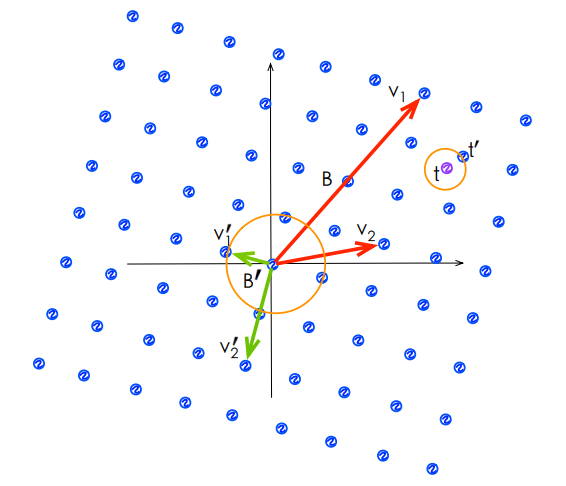
\includegraphics[width=\columnwidth]{./images/lattice.PNG}
    \end{center}
    \caption{
        Darstellung eines 2D Gitters \\ 
        \cite[Fig. 2]{xu_lighting_2018}
    }
    \label{fig:Darstellung eines 2D Gitters}
\end{figure}

Nachfolgend wird das \ac{lwe}-Problem genauer erläutert. Gegeben sei ein Vektor $s$, der den geheimen Schlüssel darstellt, und ein Vektor $e$, der den Fehler darstellt. 
Das \ac{lwe}-Problem besteht darin, den geheimen Vektor $s$ aus einer Reihe von Gleichungen der Form 
$$c = (a * s + e)\mod{q}$$ zu erlernen, wobei $c$ der Ciphertext und $a$ ein öffentlicher Vektor ist. 
Das Modulo $q$ repräsentiert eine endliche Gruppe, in der die Rechenoperationen durchgeführt werden.

Um das \ac{lwe}-Problem zu lösen, werden eine Reihe von Gleichungen erzeugt. Der geheime Vektor $s$ und der Fehlervektor $e$ werden zufällig generiert. Der öffentliche Vektor $a$ wird ebenfalls zufällig gewählt. Für jeden Gitterpunkt $i$ wird die Gleichung 
$$c_i = (a * s_i + e_i) \mod{q}$$ 
erstellt.

Der Angreifer erhält eine Menge von Gleichungen, bestehend aus den Ciphertexts $c_i$ und den öffentlichen Vektoren $a_i$. Das Ziel des Angreifers ist es, den geheimen Vektor $s_i$ zu erlernen, basierend auf den Ciphertexts und den öffentlichen Vektoren. Dies erfordert die Bestimmung der Werte des geheimen Vektors $s_i$ trotz des Vorhandenseins von Fehlern $e_i$.

Die Schwierigkeit des \ac{lwe}-Problems beruht darin, die Werte des geheimen Vektors $s_i$ aus den gegebenen Gleichungen zu rekonstruieren. Der Angreifer muss die richtigen Werte des geheimen Vektors, von den fehlerbehafteten Gleichungen unterscheiden können. Daher ist es von zentraler Bedeutung, dass die fehlerbehafteten Gleichungen ausreichend komplex sind, um eine effektive Lösung des \ac{lwe}-Problems zu verhindern.\\

Im Bereich Performance ist die Lattice-Kryptographie schneller als herkömmliche asymmetrische Verfahren, wie beispielsweise RSA. Das liegt u.a. daran, dass bei Gittern mit vergleichsweise kleinen Zahlen gearbeitet wird. Der aktuelle Stand der Technik in der gitterbasierten Kryptographie basiert hauptsächlich auf einfachen Operationen mit Matrizen und Vektoren in Ringen oder Feldern mit geringer Ordnung. So konnte bereits die Lattice-Kryptographie im Embedded Bereich auf einem 8 Bit AVR Mikrokontroller erfolgreich implementiert werden \cite*[Abs. 3]{wang_lattice-based_2023}.

% notes
%Zwei gute Vektoren, welche das Gitter bilden. Einen Punkt c durch Linearkombination finden.
%Zwei schlechte Vektoren können das selbe Gittern bilden.
%Man bekommt nur die Vektoren gegeben, nicht das Gitter.
%Wenn man eine Nachricht vershcicken möchte, wählt man einen Gitterpunkt (dieser beinhaltet einen Schlüssel). Man fügt ein Rauschen hinzu,
%sodass der Nachrichtenpunkt nur nahe dran liegt. Person A und B teilen das Gitter mit schlechten Vektoren öffentlich. 
%Closest Vector Problem im 1000-Dim Raum -> Welcher Gitter Punkt, ist am nähsten zum Nachrichtenpunkt.
%Ohne gute Vektoren im 1000dim Raum sehr schwer, selbst für QC.
